\chapter{Test on EEG measurements}\label{ch:eeg_test}
Through this chapter a modification of the main algorithm will be described such that the main algorithm can handled real EEG measurements. 

For verification of the results the MSE values achieved from the EEG measurements will be compared to MSE values achieved from the use of ICA, cf. appendix. This would include some preprocessing of the used EEG measurements.

At last, from the observed results of the comparison a conclusion will close this chapter.\\
Context of the chapter:\todo{update introduction}
\begin{itemize}
\item Description of EEG data
\item Describtion of performance measure method (practise of the Comparison to ICA) concluded by a new flow diagram.
\item Test and conclusion, including the flaws of the ICA comparison and lack of good estimate of A.
\item Description of different test approach, with different pros,including integrational functionality/connectivity(or something similar which is mentioned in ch 1.)
\item test and conclusion. 
\end{itemize}

\section{Data Description}
For this thesis a set of real EEG scalp measurements has been provided, from the the department of .... at AAU. 
The data base consist of 6 set of EEG measurements. For each of three test subjects two data set is provided, one where the test subject sit still with open eyes and one similar but with closed eyes.  
For the measurements an EEG cap with $32$ sensors measuring the scalp EEG signal with sample frequency at $512$Hz\todo{tjek sample frequency ant time} over a period of $XX$ seconds, resulting in $L = XX$ samples. That is 27 channels with names and position available in EEG.chanlocs structure\todo{Matlab eller python her?}.   
Before the data base was provided each raw data set had undergone the following preprocessing.
The data was bandpass filtered between 1 and 40 Hz. Then decomposed by ICA where the independent components related to eye activity or movement was removed. Thus, for every data set 27 sensors remains. 

One data set then consist solely of the measurement matrix $\mathbf{Y} \in \mathbb{R}^{27\times ??}$. The data set is then ready to be divided in segments for which a source matrix $\hat{\textbf{X}}$ is to be estimated by the main algorithm described in chapter \ref{ch:implementation}.

\section{Test Description}
The test procedure is now described through specification of the evaluation criteria and the practical implementation of the test.
Remember that the aim of the developed main algorithm is to estimated the source matrix in the case where the number of sensors is less than the number of active source signals -- $M<k\leq N.$.

\subsection{Performance Evaluation by Comparison to ICA}
From the description of ICA used on EEG measurements, cf. section \ref{sec:ICAsolution} ICA are considered unreliable when using low-density EEG equipment where $M<32$, but for $M\geq 32$ the currently considered the most reliably method for the source estimation. However note again that the true number of sources is not known thus there is always some unreliability to the result. 

From the view that the sources found by ICA where $N=M$ is the best estimate, it is possible to let that estimate serve as a reference to be compared to the estimates achieved when $M<N$. 
In practice that is to perform ICA on a data set $\textbf{Y}\in \mathbb{R}^{M \times L}$ resulting in $\hat{\textbf{X}}_{ICA}\in \mathbb{R}^{N\times L}$ where $M=N$, then a specific number of sensors are removed from the data set $\textbf{Y}$ such that $M<N$ then and $\hat{\textbf{X}}_{Main}\in \mathbb{R}^{N\times L}$ is estimated by the main algorithm. Then the performance of the main algorithm can be measured by comparison to the $\hat{\textbf{X}}_{ICA}$ -- does the main algorithm manage to find the same active sources as ICA, but for $M<N$?

In appendix \ref{app:ica_test}the ICA algorithm is verified on synthetic data without noise. It is found that ICA manage to estimate $\textbf{X}$ almost exact, when $M=N=k$. Furthermore it is seen that for $k < N$ ICA manage to estimate the zero rows as zero. This supports that the estimate by ICA can serve as a reference.     

To compare the two estimates the MSE, cf. section \ref{sec:mse}, is used. 
However an issue arise due to the fact that ICA do not manage to localise each of the found sources. That is the row of $\hat{\textbf{X}}_{ICA}$ do not correspond to the true $\textbf{X}$. Furhtermore the ICA algorithm is invariant toward phase and amplitude. This must necessarily worsen the resulting MSE.  

The issue is cover in appendix \ref{app:ica_test}. Here a function is considered, which manage to pair and fit the rows with the lowest mutual MSE an then arrange the rows of $\hat{\textbf{X}}_{ICA}$ such that $MSE(\textbf{X},\hat{\textbf{X}}_{ICA})$ is minimised. The fitting consist of a possible phase shift and scaling of the the amplitude.   
However this function have not been applied for this test as it as .... 

\subsection{Test Setup}
The test set up is visualised in figure \ref{fig:flow2} by a flow diagram, showing the essential steps of the test. 

\begin{figure}[H]
    \centering
	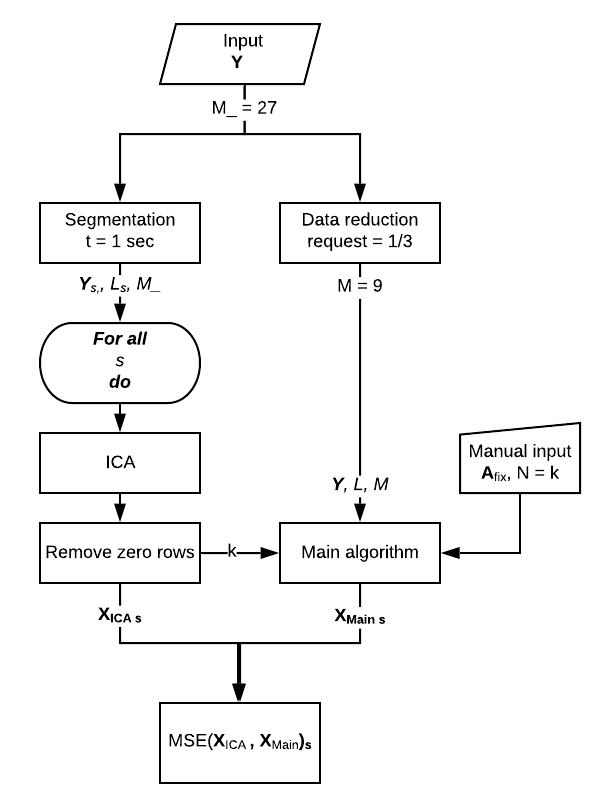
\includegraphics[scale=0.8]{figures/ch_7/flow2.png}
	\caption{Flow diagram for visualisation of the test procedure for one data set. Example given for $M<N$ where \texttt{request = 1/3} result in $M=9$.}
	\label{fig:flow2}
\end{figure}

%%% describtion of the flowchart - remainings
The ICA algorithm take the measurement matrix $\mathbf{Y}_s \in \mathbb{R}^{M \times L_s}$ for each segment $s$ as input and produced a source matrix $\mathbf{X}_s \in \mathbb{R}^{N \times L_s}$ for each segment $s$. Remember that the number of sensors equal the number of sources, $M = N$, but as mentioned in chapter XX, the case of interest are the active sources $k$, and by that $N = k$. 
For each source matrix $\mathbf{X}_s$ one need to find the $k$ active sources but it is not as easy as one may have though. Each entries of the sources matrix are to small to be detected from being active (non-zero) or being non-active (zeros).
Instead a tolerance is defined for which values less will be determined as zeros. As the source matrices have positive and negative values a tolerance interval, an interval around zero, must be made. Let the tolerance be defined as tol = $[10E-03, -10E-03]$ where values inside this interval is set equal to zero.
A problem occur in form of the stationarity of the sources as described in the motivation chapter \ref{ch:} sources are stationary if you look at small enough interval. For one second interval this is not the case with our EEG measurements and one can therefore not have a entire row (source) which laid the tolerance interval. One could decrease the length of the segments but one must also take in mind that smaller segments lead to more segments and therefore a higher computational complexity. Instead an average is introduced. For each rows (the sources) of each segments will be average such that one source is resembled by one average value. This average value will then be compared to the interval. If the value laid inside the tolerance interval, the whole row will be set equal to zero. The sources in each segment equal to zero are removed and the source matrix will now be of size $\mathbf{X}_s \in \mathbb{R}^{k \times L_s}$.

As mentioned only the sensors $M$ is known from the EEG measurement data sets but with the source matrices achieved from the ICA algorithm $k$ is now known for each segment. One now have all the information need to used the main algorithm on the EEG measurement data sets. 

S1\_Cclean is divided into 144 segments (0ne second long), with 27 sensor and 515 samples each (144 x 27 x 515).  X is found from ICA and is of size 144 x 27 x 513. X\_nonzero is X from ICA consisting of only active sources (144 x k x 513) where k is different for each segment (k is 144 long). The nonzero values if found from a tolerance of 10E-03 and -10E-03 such that at box around zero is equal to zero while the rests keep their original values (k). This is done by look at the average of one row and compared to the tolerance.
%%%

The described test is performed on the following three cases,
\begin{itemize}
\item \textbf{Test 0}: $M = N$ , to see the best possible result achieved by the main algorithm. 
\item \textbf{Test 1}: $M < N$ every third sensor is removed. 
\item \textbf{Test 2}: $M << N$ every second sensor is removed.
\end{itemize}
For each case the test is performed on one data set -- \texttt{S1\_Cclean} 

\section{Results}


\subsection{Case 0, $M = N$}
ICA is applied on $\mathbf{Y}_s$ specified by $M\_ = 27$ and $L_s = 516$. 
The main algorithm is applied on $\mathbf{Y}_s$ without any reduction hence specified by $M = 27$ and $L_s = 516$, given $\hat{\mathbf{A}}_{\text{fix}}$ and $N = k$ provided from ICA.
Figure \ref{fig:M=N_1} show $\text{MSE}\left(\hat{\mathbf{X}}_{\text{main}},\hat{\mathbf{X}}_{\text{ICA}}\right)$ for all segments $s$. 
Figure \ref{fig:M=N_1_2} show the same plot but the y-axis is specified to the interval $[-10,50]$ for better visualization.
Furthermore, the MSE tolerance $= 5$ is visualized, indicting for each segment whether the estimate $\hat{\mathbf{X}}_{\text{main}}$ is sufficiency close to $\hat{\mathbf{X}}_{\text{ICA}}$. 
For a majority of the segments the MSE lies under the tolerance, but single outliers appears for which the MSE of the segment is significantly increased. Taking the average over all segments the average achieved MSE is $5.17$.    
\begin{figure}[H]
\begin{widepage}
    \begin{minipage}[t]{.45\textwidth}
		\centering
		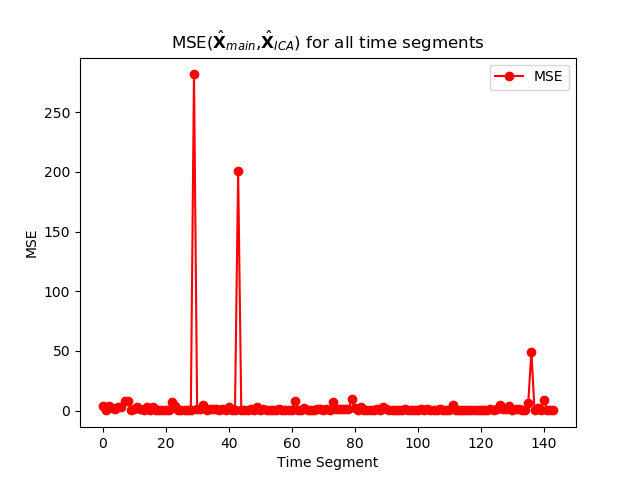
\includegraphics[width=1\linewidth]{figures/ch_7/resultat/average_mse_none_removed_ica}
	\caption{$\text{MSE} \left(\hat{\mathbf{X}}_{\text{main}}, \hat{\mathbf{X}}_{\text{ICA}}\right)$ for all $n_{\text{seg}} = $ 144 segments.}
	\label{fig:M=N_1}
    \end{minipage} 
    \hspace{0.5cm}
    \begin{minipage}[t]{.45\textwidth}
        \centering
		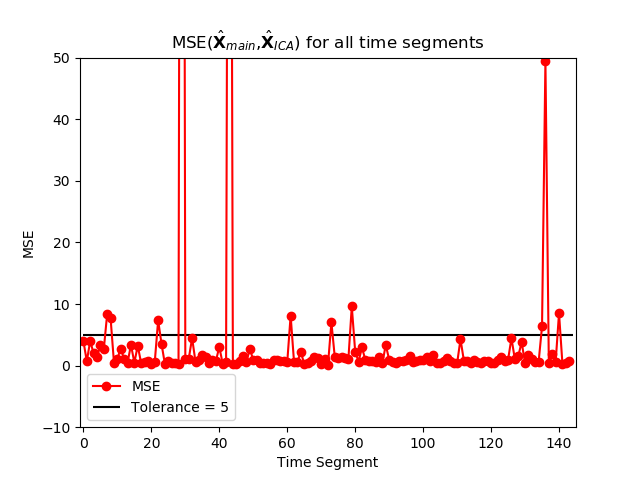
\includegraphics[width=1\linewidth]{figures/ch_7/resultat/average_mse_none_removed_ica_zoom.png}
	\caption{$\text{MSE} \left(\hat{\mathbf{X}}_{\text{main}}, \hat{\mathbf{X}}_{\text{ICA}}\right)$ for all $n_{\text{seg}} = $ 144 segments. Visualized only for the y-axis interval $[-10, 50]$ for better visualization.}
	\label{fig:M=N_1_2}
    \end{minipage}
\end{widepage}
\end{figure}
\noindent
To investigate the behavior of a single segment figure \ref{fig:M=N_2} show the MSE value computed for each row of the two estimates of a specific segment. 
That is MSE$(\hat{\mathbf{X}}_{\text{main}_{i}}$, $\hat{\mathbf{X}}_{\text{ICA}_{i}})$ for every row $i = 1, \dots, k$ in time segment $s = 5$. 
Additionally figure \ref{fig:M=N_3} show and compare the corresponding estimates for four random chosen sources. 
This allows for visual comparison of the estimates relative to the corresponding MSE value seen in figure \ref{fig:M=N_2}. 
Note that for better visual comparison each visualized row of $\hat{\mathbf{X}}_{\text{ICA}}$ is scaled with respect to the max value of the corresponding row in $\hat{\mathbf{X}}_{\text{main}}$.
From figure \ref{fig:M=N_2} it is seen that the estimate of each source result in a relative low MSE. This indicates that the main algorithm has managed to estimate the same source as the ICA algorithm. 
In contradiction to this, figure \ref{fig:M=N_3} do not confirm that the estimates are close, as generally the two signals does not follow the same trend.   
\begin{figure}[H]
\begin{widepage}
    \begin{minipage}[t]{.45\textwidth}
\centering
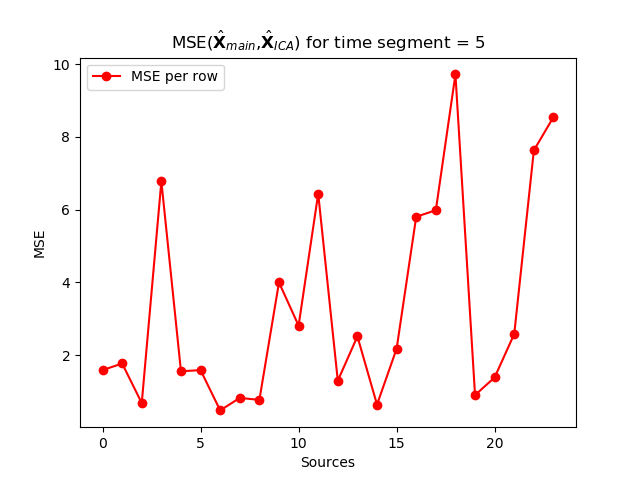
\includegraphics[width=1\linewidth]{figures/ch_7/resultat/mse_none_removed_ica_timeseg5.png}
\caption{MSE$\left(\hat{\mathbf{X}}_{\text{main}_{i}},\hat{\mathbf{X}}_{\text{ICA}_{i}}\right)$ for every row $i = 1, \dots, k$ in time segment $s=5$.}
\label{fig:M=N_2}
\end{minipage} 
\hspace{0.5cm}
\begin{minipage}[t]{.45\textwidth}
\centering
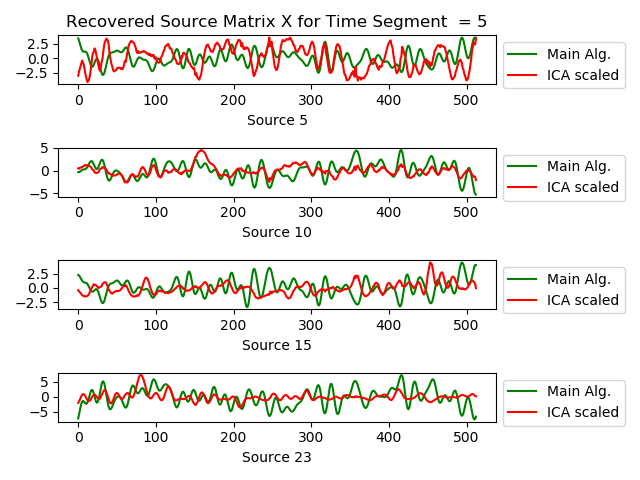
\includegraphics[width=1\linewidth]{figures/ch_7/resultat/EEG_none_removed_scaled_timeseg5S1_CClean.png}
\caption{Figure comparing four random chosen rows from $\hat{\mathbf{X}}_{\text{main}}$ and $\hat{\mathbf{X}}_{\text{ICA}}$ from time segment $s = 5$ with $M = N$ and $k=23$. Note $\hat{\mathbf{X}}_{\text{ICA}}$ is scaled for better visualization.}
	\label{fig:M=N_3}
    \end{minipage}
\end{widepage}
\end{figure}
\noindent
The test is repeated for every data set, and the results are summarized in table \ref{tab:case_0}. 
In general a low MSE is achieved in average over all segments of one data set relative to the tolerance.
And the corresponding percentage is likewise relative high, with an average at $83\%$. 
A single result is seen to deviate from the tendency, which is the data set of test subject 3 with closed eyes. 
Here a significant high average MSE value is found, indicating a majority of the segment has resulted in a significantly high MSE, while a percentage of $63\%$ was below the tolerance. 
In chapter \ref{ch:implementation} it is found that the main algorithm was capable of providing an almost exact estimate for $M = N$ when the true $\mathbf{A}$ is provided. 
Thus, it is expected that the general performance is decreased in this case where the true $\mathbf{A}$ is unknown and $\hat{\mathbf{A}}_{\text{fix}}$ is given.

The achieved results will serve as reference when analyzing the results of the following cases where the main algorithm is applied on data set with reduced number of sensors compared to the original data set.         
\begin{table}[H]
\centering
\begin{tabular}{|c|c|c|c|c|c|c|}
\hline
\multirow{2}{*}{\textbf{\begin{tabular}[c]{@{}c@{}}Case 0 \\ $M = N$\end{tabular}}} & \multicolumn{2}{c|}{Test subject 1} & \multicolumn{2}{c|}{Test subject 2} & \multicolumn{2}{c|}{Test subject 3} \\ \cline{2-7} 
                                                                                  & Open             & Close            & Open             & Close            & Open            & Close             \\ \hline
\multicolumn{1}{|c|}{Average MSE($\hat{\mathbf{X}}_{\text{ICA}},\hat{\mathbf{X}}_{\text{main}}$)}                                               & 2.913            & 5.172            & 1.572            & 15.06            & 4.753            & 19.44           \\ \hline
\begin{tabular}[c]{@{}c@{}}Segments below \\ tolerance in \%\end{tabular}          & 91             & 92            & 98 & 61             & 87            & 63 \\ \hline
\end{tabular}
\caption{Summarized results for case 0. Test is performed on the every data set.}
\label{tab:case_0}
\end{table}	
\noindent

\subsection{Case 1, $M < N$}
The main algorithm is applied on $\mathbf{Y}_s$, where the number of sensors is reduced by one-third. 
As such the main algorithm is applied on $\mathbf{Y}_s$ specified by $M = 18$ and $L_s = 516$, given $\hat{\mathbf{A}}_{\text{fix}}$ and $N = k$ provided from ICA. 
ICA is applied on the original data set with segments $\mathbf{Y}_s$ specified by $M\_ = 27$ and $L_s = 516$.  
The viewed figures correspond to those of case 0, but for the reduced number of sources $M < N$, hence detailed figure description is omitted here.   

From figure \ref{fig:M<N_1} and \ref{fig:M<N_1_2} it is seen that a majority of the segments have MSE value close to the tolerance, but the number of outliers have increased compared to case 0.
This indicates that for an increased number of segments the main algorithm do not manage to estimate enough sources sufficiently in order to stay below the tolerance. Taking the average over all segments the average achieved MSE is $5.35$.
\begin{figure}[H]
\begin{widepage}
    \begin{minipage}[t]{.45\textwidth}
		\centering
		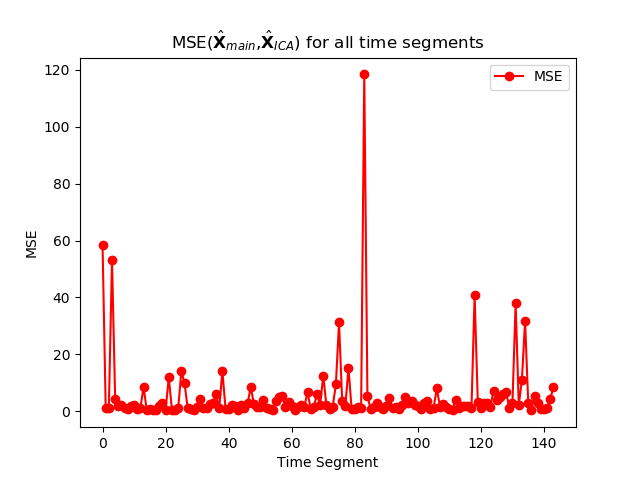
\includegraphics[width=1\linewidth]{figures/ch_7/resultat/average_mse_third_removed_ica}
	\caption{MSE$\left(\hat{\mathbf{X}}_{\text{main}},\hat{\mathbf{X}}_{\text{ICA}}\right)$ for all $n_{\text{seg}} = $ 144 segments.}
	\label{fig:M<N_1}
    \end{minipage} 
\hspace{0.5cm}
    \begin{minipage}[t]{.45\textwidth}
        \centering
		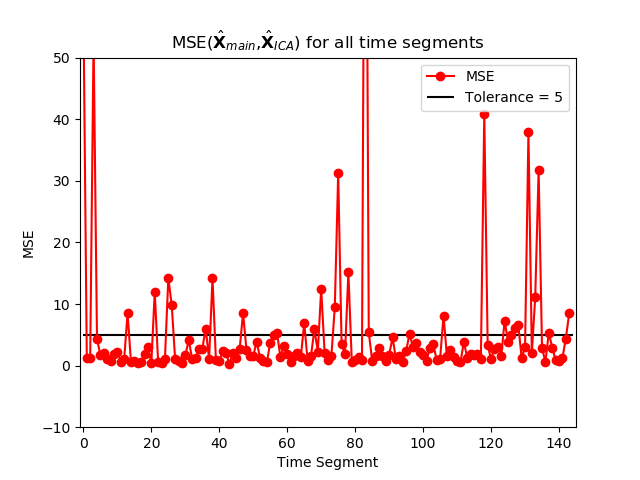
\includegraphics[width=1\linewidth]{figures/ch_7/resultat/average_mse_third_removed_ica_zoom.png}
	\caption{MSE$\left(\hat{\mathbf{X}}_{\text{main}},\hat{\mathbf{X}}_{\text{ICA}}\right)$ for all $n_{\text{seg}} = $ 144 segments. Visualized only for the y-axis interval $[-10, 50]$ for better visualization.}
	\label{fig:M<N_1_2}
    \end{minipage}
\end{widepage}
\end{figure}
\noindent 
From figure \ref{fig:M<N_2} and \ref{fig:M<N_3} showing the results of segment 5, it is seen that the MSE for each source has increased slightly compared to case 0. 
This supports the observation from figure \ref{fig:M<N_1_2}.      
\begin{figure}[H]
\begin{widepage}
    \begin{minipage}[t]{.45\textwidth}
\centering
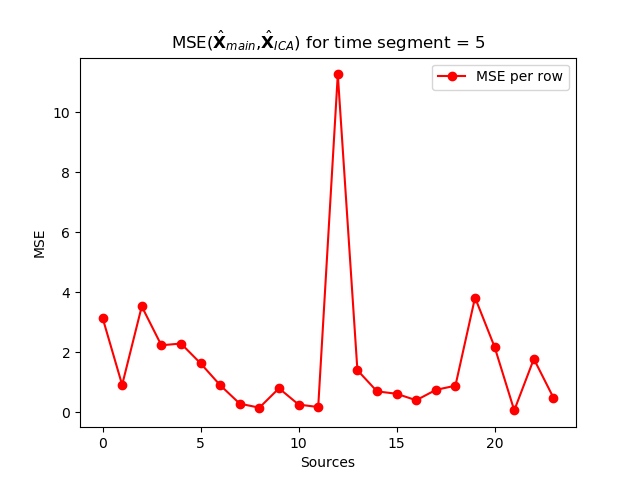
\includegraphics[width=1\linewidth]{figures/ch_7/resultat/mse_third_removed_ica_timeseg5.png}
\caption{MSE$\left(\hat{\mathbf{X}}_{\text{main}_{i}},\hat{\mathbf{X}}_{\text{ICA}_{i}}\right)$ for every row $i = 1, \dots, k$ in time segment $s=5$.}
\label{fig:M<N_2}
\end{minipage} 
\hspace{0.5cm}
\begin{minipage}[t]{.45\textwidth}
\centering
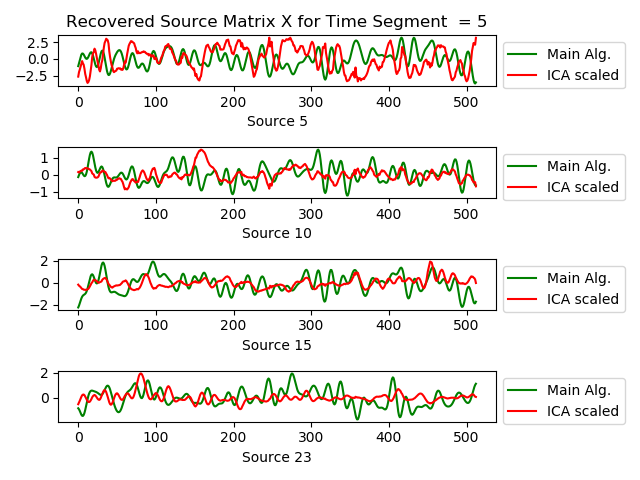
\includegraphics[width=1\linewidth]{figures/ch_7/resultat/EEG_third_removed_scaled_timeseg5S1_CClean.png}
\caption{Figure comparing four random chosen rows from $\hat{\mathbf{X}}_{\text{main}}$ and $\hat{\mathbf{X}}_{\text{ICA}}$ from time segment $s = 5$ with $M = N$ and $k=23$. Note $\hat{\mathbf{X}}_{\text{ICA}}$ is scaled for better visualization.}
	\label{fig:M<N_3}
    \end{minipage}
\end{widepage}
\end{figure}
\noindent
The test is repeated for every data set, and the results are summarized in table \ref{tab:case_1}. 
Comparing table \ref{tab:case_1} to table \ref{tab:case_0}, it is seen that the percentage of segments below the tolerance are decreasing, with the majority being close to $50\%$.
This is roughly indicating that half of the time the main algorithm do not manage to provide a sufficient estimate when $M = 2/3N$.  
Furthermore, both the average MSE and the corresponding percentages appear fluctuating relative to case 0 indicating some unreliability in the results.  
\begin{table}[H]
\centering
\begin{tabular}{|c|c|c|c|c|c|c|}
\hline
\multirow{2}{*}{\textbf{\begin{tabular}[c]{@{}c@{}}Case 1 \\ $M < N$\end{tabular}}} & \multicolumn{2}{c|}{Test subject 1} & \multicolumn{2}{c|}{Test subject 2} & \multicolumn{2}{c|}{Test subject 3} \\ \cline{2-7} 
                                                                                  & Open             & Close            & Open             & Close            & Open              & Close           \\ \hline
\multicolumn{1}{|c|}{Average MSE($\hat{\mathbf{X}}_{\text{ICA}},\hat{\mathbf{X}}_{\text{main}}$)}                                               & 9.79            & 5.351            & 13.89            & 15.13            & 6.25          & 18.21          \\ \hline
\begin{tabular}[c]{@{}c@{}}Segments below \\ tolerance in \%\end{tabular}          & 53             & 80             & 66 & 46             & 77              & 48            \\ \hline
\end{tabular}
\caption{Summarized results for case 1. Test is performed on the every data set.}
\label{tab:case_1}
\end{table}
\noindent

\subsection{Case 2, $M << N$}
The main algorithm is applied on $\mathbf{Y}_s$, where the number of sensors is reduced to half. 
As such the main algorithm is applied on $\mathbf{Y}_s$ specified by $M = 13$ and $L_s = 516$, given $\hat{\mathbf{A}}_{\text{fix}}$ and $N = k$ provided from ICA.  
ICA is applied on the original data set with segments $\mathbf{Y}_s$ specified by $M\_= 27$ and $L_s = 516$. 
The viewed figures correspond to those of case 0 and case 1, but for further reduce number of sources $M << N$, hence detailed figure description is omitted.   

From figure \ref{fig:M<<N_1} and \ref{fig:M<<N_1_2} it is seen that the MSE value for each segment is more widely scatted around the tolerance, compared to case 0 and 1. 
Outliers, where the MSE value has increased significantly, do also occur similar to case 1. 
This indicates that the performance of the main algorithm has decreased further, compared to case 1. Taking the average over all segments the average achieved MSE is $11.36$.
\begin{figure}[H]
\begin{widepage}
    \begin{minipage}[t]{.45\textwidth}
		\centering
		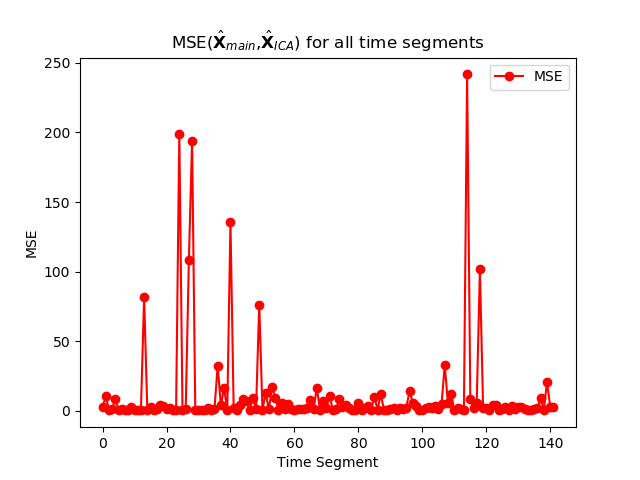
\includegraphics[width=1\linewidth]{figures/ch_7/resultat/average_mse_second_removed_ica}
	\caption{MSE$\left(\hat{\mathbf{X}}_{\text{main}},\hat{\mathbf{X}}_{\text{ICA}}\right)$ for all $n_{\text{seg}} = $ 144 segments.}
	\label{fig:M<<N_1}
    \end{minipage} 
\hspace{0.5cm}
    \begin{minipage}[t]{.45\textwidth}
        \centering
		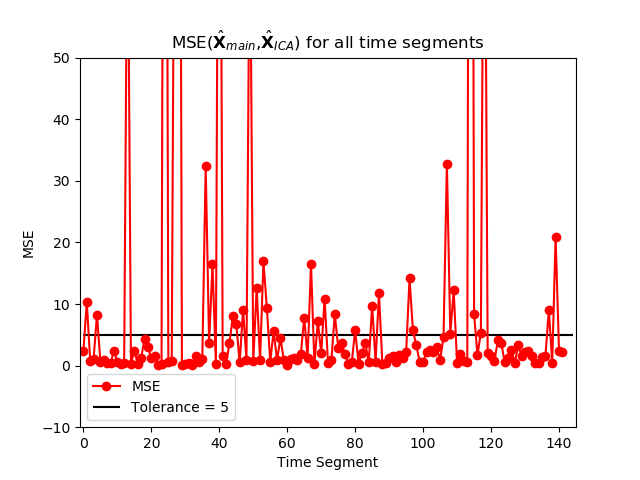
\includegraphics[width=1\linewidth]{figures/ch_7/resultat/average_mse_second_removed_ica_zoom.png}
	\caption{MSE$\left(\hat{\mathbf{X}}_{\text{main}},\hat{\mathbf{X}}_{\text{ICA}}\right)$ for all $n_{\text{seg}} = $ 144 segments. Visualized only for the y-axis interval $[-10, 50]$ for better visualization.}
	\label{fig:M<<N_1_2}
    \end{minipage}
\end{widepage}
\end{figure}
\noindent 
The above indication is supported by figure \ref{fig:M<<N_2} and \ref{fig:M<<N_3} showing an general increase in MSE. 
However, segment 5 makes a fairly good example as the majority of the sources have achieves a MSE below the tolerance of 5. 
From figure \ref{fig:M<<N_3} the increased MSE do not appear visually compared to either case 1 or case 0.        
\begin{figure}[H]
\begin{widepage}
    \begin{minipage}[t]{.49\textwidth}
\centering
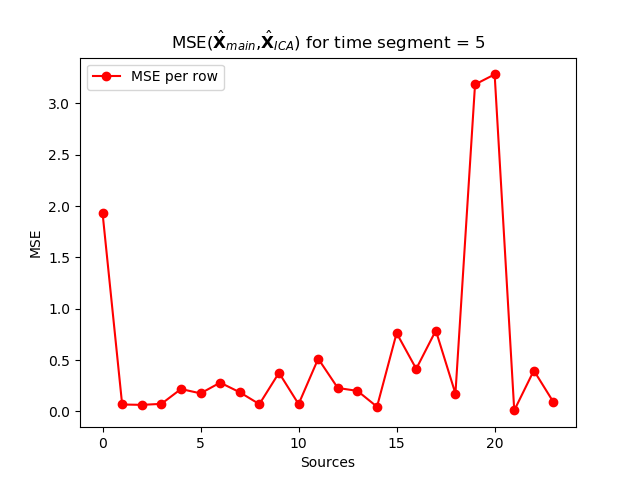
\includegraphics[width=1\linewidth]{figures/ch_7/resultat/mse_second_removed_ica_timeseg5.png}
\caption{MSE$\left(\hat{\mathbf{X}}_{\text{main}_{i}},\hat{\mathbf{X}}_{\text{ICA}_{i}}\right)$ for every row $i = 1, \dots, k$ in time segment $s = 5$.}
\label{fig:M<<N_2}
\end{minipage} 
\hspace{.5cm}
\begin{minipage}[t]{.49\textwidth}
\centering
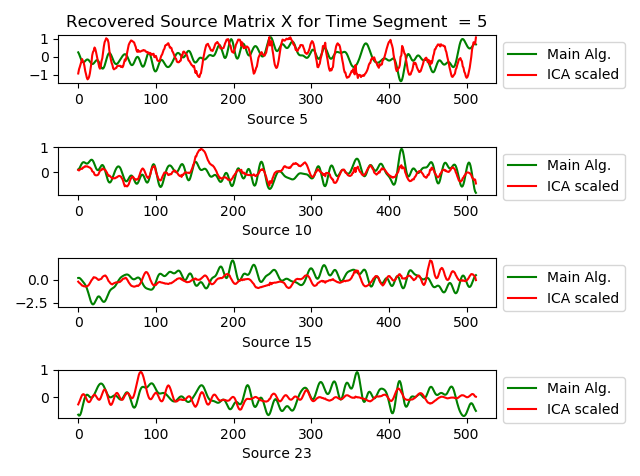
\includegraphics[width=1\linewidth]{figures/ch_7/resultat/EEG_second_removed_scaled_timeseg5S1_CClean.png}
\caption{Figure comparing four random chosen rows from $\hat{\mathbf{X}}_{\text{main}}$ and $\hat{\mathbf{X}}_{\text{ICA}}$ from time segment $s = 5$ with $M << N$ and $k=23$. Note $\hat{\mathbf{X}}_{\text{ICA}}$ is scaled for better visualization.}
	\label{fig:M<<N_3}
    \end{minipage}
\end{widepage}
\end{figure}
\noindent
The test is repeated for every data set, and the results are summarized in table \ref{tab:case_2}. Comparing table \ref{tab:case_0} to table \ref{tab:case_1} it is generally seen that the percentage of segments below the tolerance are not decreased but improved.
Though, without getting close to the tendency from case 0. 
Furthermore, the average MSE have not increased remarkably compared to case 1. 
As such the performance of the main algorithm in case 2 is in general not found to be worse than for case 1.
However, a clear improvement is not seen either.  
\begin{table}[H]
\centering
\begin{tabular}{|c|c|c|c|c|c|c|}
\hline
\multirow{2}{*}{\textbf{\begin{tabular}[c]{@{}c@{}}Case 2\\ $M << N$\end{tabular}}} & \multicolumn{2}{c|}{Test subject 1} & \multicolumn{2}{c|}{Test subject 2} & \multicolumn{2}{c|}{Test subject 3} \\ \cline{2-7} 
                                                                                  & Open             & Close            & Open             & Close            & Open             & Close            \\ \hline
\multicolumn{1}{|c|}{Average MSE($\hat{\mathbf{X}}_{\text{ICA}},\hat{\mathbf{X}}_{\text{main}}$)}                                               & 8.378            & 11.36            & 19.58            & 13.11            & 13.99           & 11.96            \\ \hline
\begin{tabular}[c]{@{}c@{}}Segments below \\ tolerance in \%\end{tabular}          & 75             & 74             & 42 & 72             & 69             & 69 \\ \hline
\end{tabular}
\caption{Summarized results for case 2. Test is performed on the every data set.}
\label{tab:case_2}
\end{table}
\noindent


\section{Conclusion}